\documentclass[9pt,lineno]{elife}

% graphicx package, useful for including eps and pdf graphics
\usepackage{graphicx}
\DeclareGraphicsExtensions{.png,.png,.jpg}

% basic packages
\usepackage{color}
\usepackage{parskip}
\usepackage{float}
\usepackage{microtype}
\usepackage{url}
\usepackage{hyperref}
\usepackage{booktabs}
\usepackage{makecell}
\usepackage{multirow}

% text layout
\usepackage{geometry}
\geometry{textwidth=17cm} % 15.25cm for single-space, 16.25cm for double-space
\geometry{textheight=22.5cm} % 22cm for single-space, 22.5cm for double-space

% helps to keep figures from being orphaned on a page by themselves
\renewcommand{\topfraction}{0.85}
\renewcommand{\textfraction}{0.1}

% bold the 'Figure #' in the caption and separate it with a period
% Captions will be left justified
\usepackage[labelfont=bf,labelsep=period,font=small]{caption}

% cite package, to clean up citations in the main text. Do not remove.
%\usepackage{cite}
%\usepackage{natbib}

%% \usepackage{lineno}
%% \linenumbers

\usepackage{authblk}
\renewcommand\Authands{ \& }
\renewcommand\Authfont{\normalsize \bf}
\renewcommand\Affilfont{\small \normalfont}
\makeatletter
\renewcommand\AB@affilsepx{, \protect\Affilfont}
\makeatother

% latexdiff

%DIF UNDERLINE PREAMBLE %DIF PREAMBLE
\RequirePackage[normalem]{ulem} %DIF PREAMBLE
\RequirePackage{color}\definecolor{RED}{rgb}{1,0,0}\definecolor{BLUE}{rgb}{0,0,1} %DIF PREAMBLE
\providecommand{\DIFadd}[1]{{\protect\color{blue}\uwave{#1}}} %DIF PREAMBLE
\providecommand{\DIFdel}[1]{{\protect\color{red}\sout{#1}}}                      %DIF PREAMBLE
%DIF SAFE PREAMBLE %DIF PREAMBLE
\providecommand{\DIFaddbegin}{} %DIF PREAMBLE
\providecommand{\DIFaddend}{} %DIF PREAMBLE
\providecommand{\DIFdelbegin}{} %DIF PREAMBLE
\providecommand{\DIFdelend}{} %DIF PREAMBLE
%DIF FLOATSAFE PREAMBLE %DIF PREAMBLE
\providecommand{\DIFaddFL}[1]{\DIFadd{#1}} %DIF PREAMBLE
\providecommand{\DIFdelFL}[1]{\DIFdel{#1}} %DIF PREAMBLE
\providecommand{\DIFaddbeginFL}{} %DIF PREAMBLE
\providecommand{\DIFaddendFL}{} %DIF PREAMBLE
\providecommand{\DIFdelbeginFL}{} %DIF PREAMBLE
\providecommand{\DIFdelendFL}{} %DIF PREAMBLE

% comments
%% \definecolor{purple}{rgb}{0.459,0.109,0.538}
%% \def\tbc#1{\textcolor{purple}{[#1]}}
%% \def\rnc#1{\textcolor{blue}{[#1]}}
\def\jhc#1{\textcolor{red}{[#1]}}

\title{Genetic cartography reveals ancestral relationships of human pathogenic viruses}

\author[1]{Sravani Nanduri}
\author[2]{John Huddleston}
\author[2]{Allison Black}
\author[2*]{Trevor Bedford}

\affil[1]{Issaquah High School, Issaquah, WA, USA}
\affil[2]{Vaccine and Infectious Disease Division, Fred Hutchinson Cancer Research Center, Seattle, WA, USA}

\corr{trevor@bedford.io}{TB}

\date{}

\begin{document}
\maketitle

\begin{abstract}
\end{abstract}

\section*{Introduction}

Tracking the evolution of human pathogenic viruses in real time enables epidemiologists to respond quickly to emerging epidemics and local outbreaks.
Real-time analyses of viral evolution typically rely on phylogenetic methods.
These methods can reconstruct the evolutionary history of viral populations from their genome sequences and estimate states of inferred ancestral viruses including their most likely genome sequence, time of circulation, and geographic location (gen epi papers).
Importantly, these methods assume that all sequence data share an evolutionary history represented by the clonal replication of genomes.
In practice, the evolutionary histories of many human pathogenic viruses including seasonal influenza viruses, Zika virus, and coronaviruses violate this assumption through processes of recombination or reassortment.
Researchers have attempted to compensate for these evolutionary mechanisms by limiting their analyses to specific genes (citation?), concatenating multiple genes despite their different evolutionary histories (citation?), or developing more sophisticated models to represent the joint likelihoods of multiple co-evolving lineages represented by networks rather than trees (Muller).
However, several key questions in genomic epidemiology do not require full phylogenetic inference of ancestral relationships and states.
For example, genomic epidemiologists commonly need to 1) identify clusters of closely-related genomes that represent regional outbreaks or new variants of concern (Black et al.? MicrobeTrace?), 2) rapidly place newly sequenced viral genomes in the evolutionary context of other circulating strains (USHER, NextClade), and 3) flag low-quality or mislabeled genome sequences for exclusion from their analyses.
These common use cases can all be addressed by standard statistical methods including clustering, classification, and outlier detection.
These methods make few assumptions about the input data and therefore should be applicable to genomic data that violate phylogenetic assumptions.

To apply these methods to a population of viral genomes, we need metrics to compare genome sequences to each other and algorithms to reduce the highly multidimensional input data (M x N for M genomes of length N) to one or two dimensions where clustering, classification, and outlier detection are more tractable.
The number of mismatches between any pair of aligned genome sequences, also known as the Hamming distance, provides a natural distance metric for viral genomes.
Indeed, most phylogenetic methods start by building a matrix of Hamming distances between all sequences in a given multiple sequence alignment.
Many dimensionality reduction algorithms including multidimensional scaling (MDS) \citep{hout_papesh_goldinger_2012}, t-SNE \citep{maaten2008visualizing}, and UMAP \citep{lel2018umap} accept such distance matrices as an input and produce a corresponding lower-dimensional representation or “embedding” of those data.
Alternately, principal components analysis (PCA) only requires the input data to be transformed to a matrix of integers before it can embed those data into a few orthogonal dimensions.

Each of these embedding methods has been applied to genomic data to visualize relationships between individuals and identify clusters of related genomes.
PCA has been applied to single nucleotide polymorphisms (SNPs) of human genomes \citep{novembre_2008,alexander_2009,mcvean_2009,auton_2015} and to multiple sequence alignments of viral genomes \citep{metsky_2017}.
Although PCA is a generic linear algebra algorithm that optimizes for an orthogonal embedding of the data, the principal components from SNPs represent mean coalescent times and therefore recapitulate broad phylogenetic relationships \citep{mcvean_2009}.
MDS has been applied to multiple gene segments of seasonal influenza viruses to understand evolutionary relationships between segments \citep{rambaut_2008}.
MDS attempts to embed input data into a lower-dimensional representation such that each pair of data points are as far apart in the embedding as they are in the original data.
Modern embedding methods like t-SNE and UMAP have also been applied to SNPs from human genomes \citep{diaz-papkovich_2019} and single-cell transcriptomes \citep{becht_2018,kobak_2019}.
t-SNE and UMAP build on manifold learning methods like MDS to find low-dimensional embeddings of data that place similar points close together and dissimilar points far apart \citep{kobak_2021}.

Although these embedding methods are commonly used for qualitative studies of evolutionary relationships, few studies have attempted to quantify patterns observed in these embeddings and no studies have investigated the value of applying these methods to human pathogenic viruses.
To this end, we applied PCA, MDS, t-SNE, and UMAP to genomes from recent populations of seasonal influenza virus A/H3N2, Zika virus, MERS-CoV, and SARS-CoV-2.
Each of these viruses have impacted human populations globally in the last decade and have been studied in real time by genomic epidemiologists.
For each virus and embedding method, we quantified the relationship between pairwise sequence and embedding distances, identified clusters of closely-related genomes in embedding space, and evaluated the accuracy of clusters compared to expert-defined phylogenetic clades.
Finally, we tested the practical application of these methods to identify reassortment and outliers in seasonal influenza viruses.
These results inform our recommendations for future applications of these methods including which methods are most effective for specific problems in genomic epidemiology and which parameters to use for each method.

\section*{Results}

\subsection*{Embedding clusters recapitulate phylogenetic clades for seasonal influenza A/H3N2}

\subsubsection*{Model training and validation of embeddings with populations between 2016--2018}

All four dimensionality reduction methods qualitatively recapitulated clade-level groupings observed in the phylogeny (Figure~\ref{fig:seasonal-influenza-h3n2-ha-embeddings}).
Strains from the same clade appeared tightly grouped in PCA, t-SNE, and UMAP embeddings and more loosely clustered in the MDS embedding.
Closely related clades tended to tightly cluster in PCA, MDS, UMAP, and, to a lesser extent, t-SNE.
For example, the clade A2 and its subclade A2/re map to adjacent regions of all four embeddings.
We observed the same pattern for A1 and its subclade A1a as well as for A1b and its subclades A1b/135K and A1b/135N.
The clade 3c2.A and its subclade A3 clustered in all embeddings except t-SNE.
This result matched our expectation that t-SNE would preserve local clusters and not retain global structure between more distantly related data.

\begin{figure}[htb]
  \begin{center}
  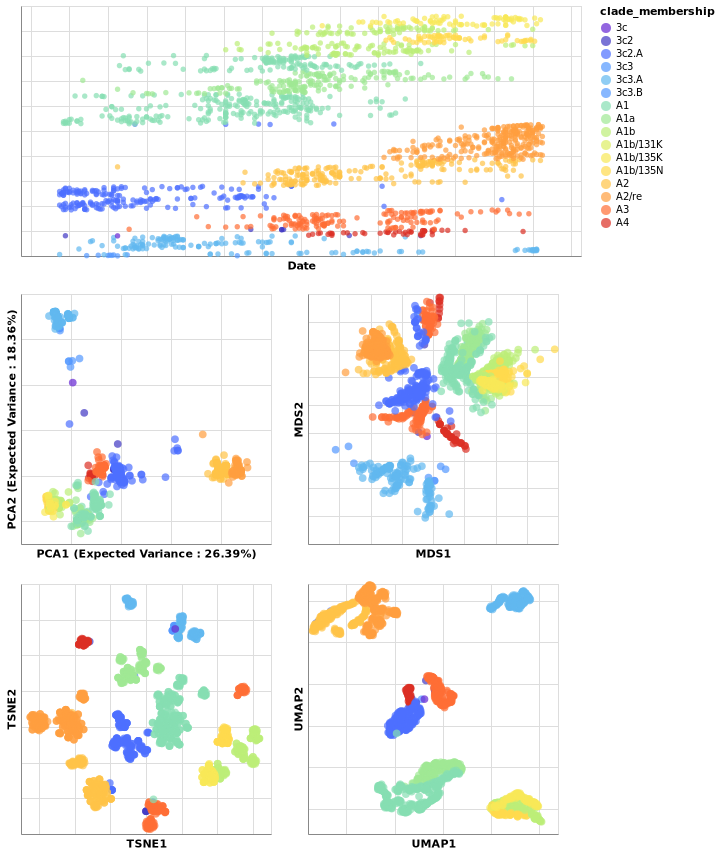
\includegraphics[width=\columnwidth]{flu-embeddings}
  \caption{
    The phylogeny of influenza A/H3N2 viruses (top) shows the evolutionary relationships among viruses including clades, or viruses that share the same mutations and descend from the same common ancestor.
    Reduced dimensionality embeddings of genetic sequences into two dimensions by PCA (middle left), MDS (middle right), t-SNE (bottom left), and UMAP (bottom right) generally recapitulate groups of viruses into clades without inferring ancestral relationships.
  }
  \label{fig:seasonal-influenza-h3n2-ha-embeddings}
  \end{center}
\end{figure}

To quantify the patterns we observed in Figure~\ref{fig:seasonal-influenza-h3n2-ha-embeddings}, we calculated two complementary metrics for each embedding method.
First, we measured the linearity of the relationship of Euclidean distance between two strains in an embedding space and the genetic distance between these same strains.
All four methods exhibited a consistent linear relationship for pairs of strains that differed by no more than 20 nucleotides (Figure~\ref{fig:seasonal-influenza-h3n2-ha-pairwise-distances}).
PCA and MDS provided the strongest linear mapping to genetic distance (Pearson's $R^{2} = 0.767 \pm 0.000$  and $0.849 \pm 0.000$, respectively).
This same mapping for the UMAP method was less of a linear function (Pearson's $R^{2} = 0.397 \pm 0.000$) than a piecewise function of two parts.
Strain pairs with more than 30 nucleotide differences were not as well separated in UMAP space as strains with lesser genetic distances.
This result suggests that UMAP might be most effective for distinguishing between more distantly related strain pairs.
t-SNE's mapping was the weakest (Pearson's $R^{2} = 0.393 \pm 0.001$) and revealed that only closely related strains map near each other in t-SNE space.
Pairs of strains that differ by more than 15 nucleotides are unlikely to be placed near each other in a t-SNE embedding.

\begin{figure}[htb]
  \begin{center}
  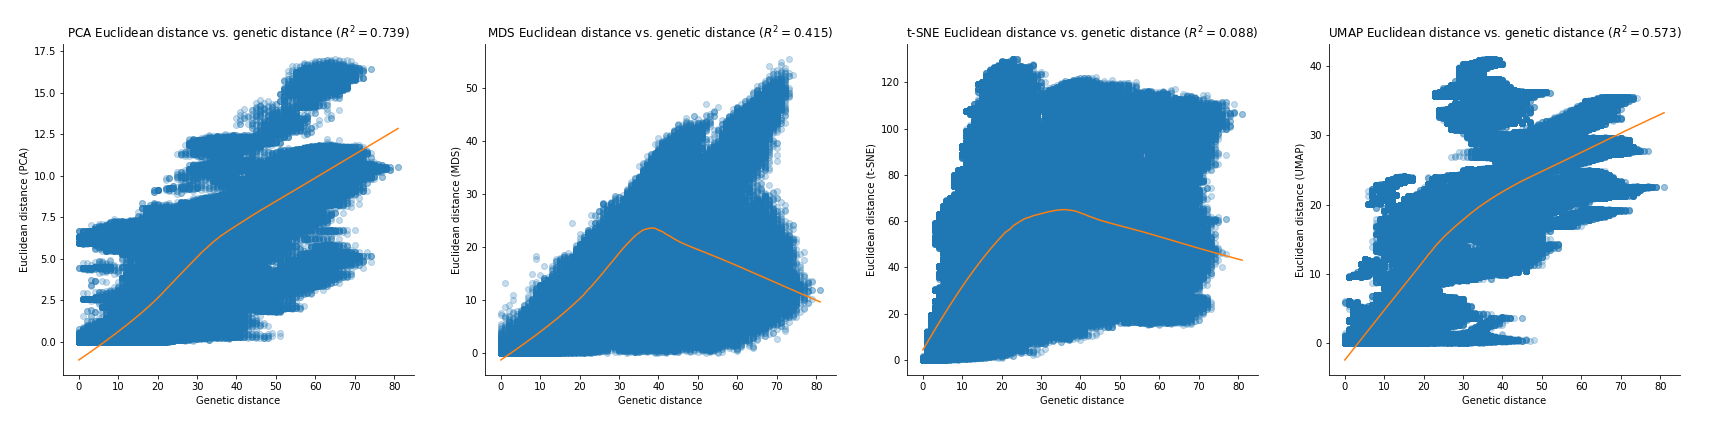
\includegraphics[width=\columnwidth]{FullScatterplotFlu.png}
  \caption{
    The mapping between Euclidean and Genetic distance assess the strength of both the local and global structure of the embedding recapitulation.
    The scatterplot for PCA (upper left), MDS (upper right), t-SNE (lower left), and UMAP (lower right) consistently exhibit linear relationships for pairs of strains that differ by around 20 nucleotides.
  }
  \label{fig:seasonal-influenza-h3n2-ha-pairwise-distances}
  \end{center}
\end{figure}

Second, we determined how accurately the Euclidean distance between pairs of strains in an embedding could classify those strains as belonging to the same clade or not.
Specifically, we used a Support Vector Machine (SVM) classifier to identify an optimal Euclidean distance threshold that distinguished pairs of strains from the same clade.
To train the classifier, we used the Euclidean distance between all pairs of strains as a one-dimensional feature and a binary encoding of within (1) or between (0) clade status as a model target.
As there were far more pairs of strains from different clades, we measured classification accuracy with the Matthew's correlation coefficient (MCC), a metric that is robust to unbalanced counts in the confusion matrix \citep{matthews_1975}.
As a control, we compared the accuracy of each method's classifier to the MCC from a classifier fit to genetic distance between strains.
t-SNE, UMAP, and PCA provided the most accurate classifications (MCC = 0.686, 0.695, 0.682, respectively) and matched or outperformed pairwise genetic distance (MCC = 0.589) (Figure~\ref{fig:seasonal-influenza-h3n2-ha-clusters}, Table~1).
MDS performed poorly (MCC = 0.54), confirming our expectations it would mirror genetic distances MCC value based on MDS's linear relationship with genetic distance.
These results show the potential benefits of using t-SNE embeddings for cluster analysis over the computationally simpler genetic distance, despite the t-SNE's lack of global linear relationships between strains.

\begin{figure}[htb]
  \begin{center}
  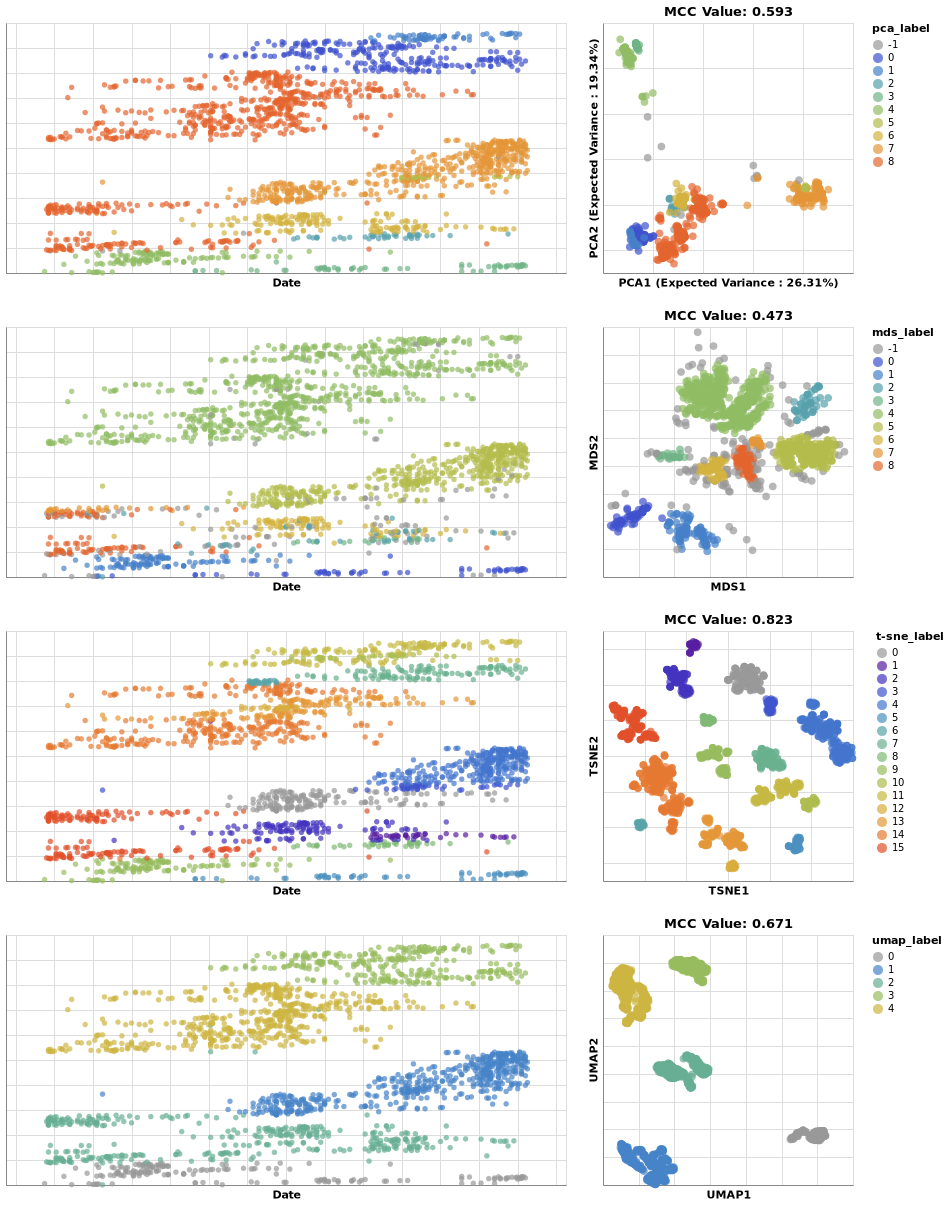
\includegraphics[width=\columnwidth]{fullHDBSCANChartFlu.png}
  \caption{
    The embeddings colored by their HDBSCAN label, with the distance threshold defined by the threshold that preserved the greatest amount of clade relationships.
    The chart for PCA (top left), MDS (middle left), t-SNE (middle left), and UMAP (bottom left) generally recapitulate groups of viruses into clades without inferring ancestral relationships, and the trees on the righthand side describes how these clade grouping appear on the tree, which does infer ancestral relations.
    \jhc{These embeddings do not match the embeddings in Figure 1. Is this based on the same data and parameters?}
  }
  \label{fig:seasonal-influenza-h3n2-ha-clusters}
  \end{center}
\end{figure}

\subsubsection*{Model testing of embeddings with populations between 2018--2020}

\subsection*{Zika virus clusters reveal geographic patterns of the 2013--2018 epidemic}

\begin{figure}[htb]
  \begin{center}
  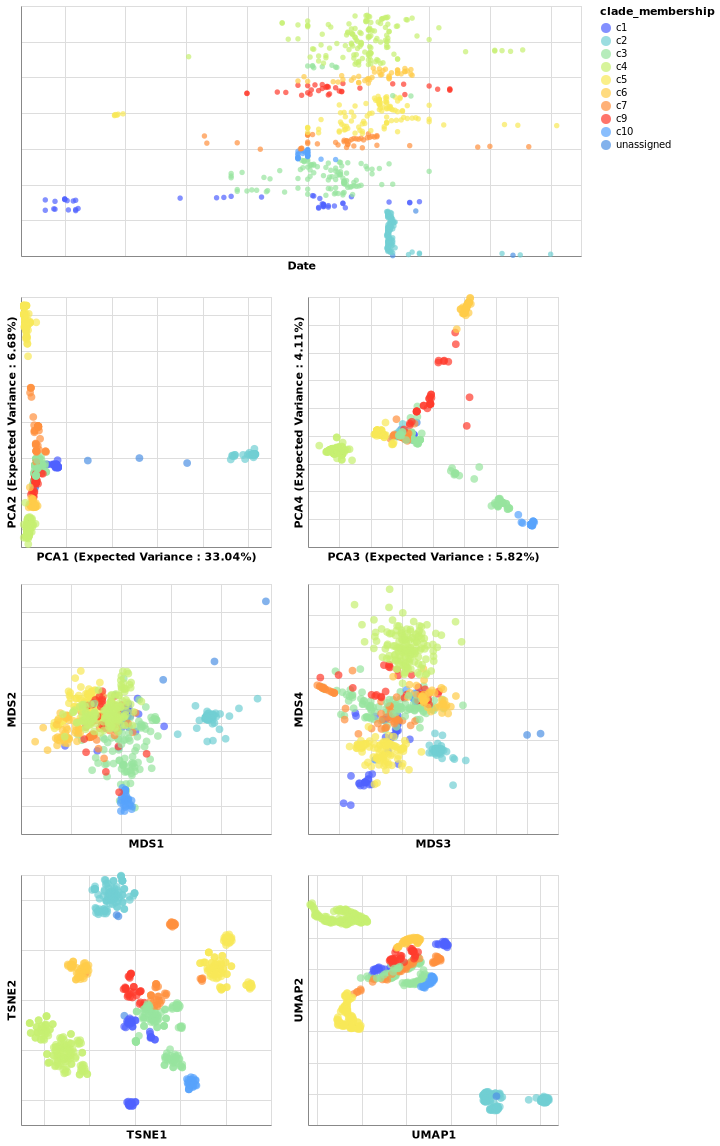
\includegraphics[width=\columnwidth]{zika-embeddings}
  \caption{
    Genetic cartography of Zika strains by dimensionality reduction methods.
    PCA (components 1 and 2 upper left, components 3 and 4 upper right), MDS (middle left and middle right), t-SNE (lower left), and UMAP (lower right) compared to inferred phylogeny (upper plot).
    PC1 and PC2 delineate the variance between the Americas and Asia, and PC3 and PC4 are included to better display the variance within the Americas.
  }
  \label{fig:zika-embeddings}
  \end{center}
\end{figure}

All four dimensionality reduction methods recapitulated phylogenetic patterns observed in the phylogeny (Figure~\ref{fig:zika-embeddings}).
PCA, after imputing missing data, had a similar structure to the findings in Metsky et.al., where the clades were loosely clustered on a continuum of different clades instead of tightly clustered as seen in influenza.
Geographical introductions and outbreaks isolated from others were placed at larger Euclidean distances than related introductions.
An example is clade c2, an outbreak in Singapore and Thailand separated from the geographical introductions in the Americas.
Clade c10 is also a good example of a densely sampled outbreak in Colombia (introduced from Brazil) that forms distinct clusters in all the embeddings.
PC1 and PC2 delineate the variance between c2 and the other clades (variance between Asia and the Americas), and PC3 and PC4 are used to show the variance between clade c4 and c3 compared to clade c6 and c9 (variance within the Americas).
PC1 and PC2 defined clusters of outbreaks not noted in the phylogenetic tree, such as a small Brazil-only outbreak as well as a cluster from China and Samoa.
Clade c9 is a second parent of an outbreak in Brazil that spread to the US Virgin Islands and Puerto Rico, where c6 is a child outbreak that spread into neighboring countries.
All four of the embeddings recognized their relatedness and placed clades c6 and c9 in close proximity to each other.
Clade c4, a Central American outbreak that spread to Puerto Rico and other neighboring countries, was not placed closely to clades c6 and c9 even given similar geographical locations and introduction times.
This suggests that strains from the same introduction cluster together, and do not cluster just by where they were introduced.

\subsection*{MERS-CoV clusters correspond to host-specific outbreaks}

\subsection*{SARS-CoV-2 clusters recapitulate emerging lineage designations}

\subsection*{Joint embeddings of hemagglutinin and neuraminidase genomes identify seasonal influenza virus A/H3N2 reassortment events}

\subsection*{Embeddings of hemagglutinin genomes identify low-quality or misannotated seasonal influenza viruses}

\section*{Discussion}

\section*{Materials and methods}

\subsection*{Data and software availability}

The entire workflow for our analyses was implemented with Snakemake \citep{molder_2021}.
We have provided all source code, configuration files, and datasets at \href{https://github.com/blab/cartography}{https://github.com/blab/cartography}.

\section*{Acknowledgments}

\section*{Author contributions}

SN...
JH...
AB...
TB...

\section*{Competing interests}

The authors declare that no competing interests exist.

\section*{Supplemental Files}

\bibliography{cartography}

\end{document}
